\documentclass[]{article}
\usepackage{lmodern}
\usepackage{amssymb,amsmath}
\usepackage{ifxetex,ifluatex}
\usepackage{fixltx2e} % provides \textsubscript
\ifnum 0\ifxetex 1\fi\ifluatex 1\fi=0 % if pdftex
  \usepackage[T1]{fontenc}
  \usepackage[utf8]{inputenc}
\else % if luatex or xelatex
  \ifxetex
    \usepackage{mathspec}
  \else
    \usepackage{fontspec}
  \fi
  \defaultfontfeatures{Ligatures=TeX,Scale=MatchLowercase}
\fi
% use upquote if available, for straight quotes in verbatim environments
\IfFileExists{upquote.sty}{\usepackage{upquote}}{}
% use microtype if available
\IfFileExists{microtype.sty}{%
\usepackage{microtype}
\UseMicrotypeSet[protrusion]{basicmath} % disable protrusion for tt fonts
}{}
\usepackage[margin=1in]{geometry}
\usepackage{hyperref}
\hypersetup{unicode=true,
            pdftitle={Statistical Inference: Toothgrowth experiment},
            pdfauthor={Sanjay Somraj},
            pdfborder={0 0 0},
            breaklinks=true}
\urlstyle{same}  % don't use monospace font for urls
\usepackage{color}
\usepackage{fancyvrb}
\newcommand{\VerbBar}{|}
\newcommand{\VERB}{\Verb[commandchars=\\\{\}]}
\DefineVerbatimEnvironment{Highlighting}{Verbatim}{commandchars=\\\{\}}
% Add ',fontsize=\small' for more characters per line
\usepackage{framed}
\definecolor{shadecolor}{RGB}{248,248,248}
\newenvironment{Shaded}{\begin{snugshade}}{\end{snugshade}}
\newcommand{\KeywordTok}[1]{\textcolor[rgb]{0.13,0.29,0.53}{\textbf{{#1}}}}
\newcommand{\DataTypeTok}[1]{\textcolor[rgb]{0.13,0.29,0.53}{{#1}}}
\newcommand{\DecValTok}[1]{\textcolor[rgb]{0.00,0.00,0.81}{{#1}}}
\newcommand{\BaseNTok}[1]{\textcolor[rgb]{0.00,0.00,0.81}{{#1}}}
\newcommand{\FloatTok}[1]{\textcolor[rgb]{0.00,0.00,0.81}{{#1}}}
\newcommand{\ConstantTok}[1]{\textcolor[rgb]{0.00,0.00,0.00}{{#1}}}
\newcommand{\CharTok}[1]{\textcolor[rgb]{0.31,0.60,0.02}{{#1}}}
\newcommand{\SpecialCharTok}[1]{\textcolor[rgb]{0.00,0.00,0.00}{{#1}}}
\newcommand{\StringTok}[1]{\textcolor[rgb]{0.31,0.60,0.02}{{#1}}}
\newcommand{\VerbatimStringTok}[1]{\textcolor[rgb]{0.31,0.60,0.02}{{#1}}}
\newcommand{\SpecialStringTok}[1]{\textcolor[rgb]{0.31,0.60,0.02}{{#1}}}
\newcommand{\ImportTok}[1]{{#1}}
\newcommand{\CommentTok}[1]{\textcolor[rgb]{0.56,0.35,0.01}{\textit{{#1}}}}
\newcommand{\DocumentationTok}[1]{\textcolor[rgb]{0.56,0.35,0.01}{\textbf{\textit{{#1}}}}}
\newcommand{\AnnotationTok}[1]{\textcolor[rgb]{0.56,0.35,0.01}{\textbf{\textit{{#1}}}}}
\newcommand{\CommentVarTok}[1]{\textcolor[rgb]{0.56,0.35,0.01}{\textbf{\textit{{#1}}}}}
\newcommand{\OtherTok}[1]{\textcolor[rgb]{0.56,0.35,0.01}{{#1}}}
\newcommand{\FunctionTok}[1]{\textcolor[rgb]{0.00,0.00,0.00}{{#1}}}
\newcommand{\VariableTok}[1]{\textcolor[rgb]{0.00,0.00,0.00}{{#1}}}
\newcommand{\ControlFlowTok}[1]{\textcolor[rgb]{0.13,0.29,0.53}{\textbf{{#1}}}}
\newcommand{\OperatorTok}[1]{\textcolor[rgb]{0.81,0.36,0.00}{\textbf{{#1}}}}
\newcommand{\BuiltInTok}[1]{{#1}}
\newcommand{\ExtensionTok}[1]{{#1}}
\newcommand{\PreprocessorTok}[1]{\textcolor[rgb]{0.56,0.35,0.01}{\textit{{#1}}}}
\newcommand{\AttributeTok}[1]{\textcolor[rgb]{0.77,0.63,0.00}{{#1}}}
\newcommand{\RegionMarkerTok}[1]{{#1}}
\newcommand{\InformationTok}[1]{\textcolor[rgb]{0.56,0.35,0.01}{\textbf{\textit{{#1}}}}}
\newcommand{\WarningTok}[1]{\textcolor[rgb]{0.56,0.35,0.01}{\textbf{\textit{{#1}}}}}
\newcommand{\AlertTok}[1]{\textcolor[rgb]{0.94,0.16,0.16}{{#1}}}
\newcommand{\ErrorTok}[1]{\textcolor[rgb]{0.64,0.00,0.00}{\textbf{{#1}}}}
\newcommand{\NormalTok}[1]{{#1}}
\usepackage{graphicx,grffile}
\makeatletter
\def\maxwidth{\ifdim\Gin@nat@width>\linewidth\linewidth\else\Gin@nat@width\fi}
\def\maxheight{\ifdim\Gin@nat@height>\textheight\textheight\else\Gin@nat@height\fi}
\makeatother
% Scale images if necessary, so that they will not overflow the page
% margins by default, and it is still possible to overwrite the defaults
% using explicit options in \includegraphics[width, height, ...]{}
\setkeys{Gin}{width=\maxwidth,height=\maxheight,keepaspectratio}
\IfFileExists{parskip.sty}{%
\usepackage{parskip}
}{% else
\setlength{\parindent}{0pt}
\setlength{\parskip}{6pt plus 2pt minus 1pt}
}
\setlength{\emergencystretch}{3em}  % prevent overfull lines
\providecommand{\tightlist}{%
  \setlength{\itemsep}{0pt}\setlength{\parskip}{0pt}}
\setcounter{secnumdepth}{0}
% Redefines (sub)paragraphs to behave more like sections
\ifx\paragraph\undefined\else
\let\oldparagraph\paragraph
\renewcommand{\paragraph}[1]{\oldparagraph{#1}\mbox{}}
\fi
\ifx\subparagraph\undefined\else
\let\oldsubparagraph\subparagraph
\renewcommand{\subparagraph}[1]{\oldsubparagraph{#1}\mbox{}}
\fi

%%% Use protect on footnotes to avoid problems with footnotes in titles
\let\rmarkdownfootnote\footnote%
\def\footnote{\protect\rmarkdownfootnote}

%%% Change title format to be more compact
\usepackage{titling}

% Create subtitle command for use in maketitle
\newcommand{\subtitle}[1]{
  \posttitle{
    \begin{center}\large#1\end{center}
    }
}

\setlength{\droptitle}{-2em}
  \title{Statistical Inference: Toothgrowth experiment}
  \pretitle{\vspace{\droptitle}\centering\huge}
  \posttitle{\par}
  \author{Sanjay Somraj}
  \preauthor{\centering\large\emph}
  \postauthor{\par}
  \predate{\centering\large\emph}
  \postdate{\par}
  \date{March 23, 2017}


\begin{document}
\maketitle

\section{Statistical Inference Course Project - PART
2}\label{statistical-inference-course-project---part-2}

\subsection{Overview}\label{overview}

Load the ToothGrowth data and perform some basic exploratory data
analyses\\
a) Provide a basic summary of the data.\\
b) Use confidence intervals and/or hypothesis tests to compare tooth
growth by supp and dose.\\
(Only use the techniques from class, even if there's other approaches
worth considering)\\
c) State your conclusions and the assumptions needed for your
conclusions.

\subsection{Load libraries}\label{load-libraries}

\begin{Shaded}
\begin{Highlighting}[]
\CommentTok{# Load libraries for data processing and plotting}
\KeywordTok{library}\NormalTok{(ggplot2)}
\KeywordTok{library}\NormalTok{(datasets)}
\KeywordTok{library}\NormalTok{(gridExtra)}
\KeywordTok{library}\NormalTok{(grid)}

\CommentTok{# The Effect of Vitamin C on Tooth Growth in Guinea Pigs}
\KeywordTok{data}\NormalTok{(ToothGrowth)}
\end{Highlighting}
\end{Shaded}

\subsection{Basic Summary of the data}\label{basic-summary-of-the-data}

\begin{Shaded}
\begin{Highlighting}[]
\CommentTok{# Structure of the data frame}
\KeywordTok{str}\NormalTok{(ToothGrowth)}
\end{Highlighting}
\end{Shaded}

\begin{verbatim}
## 'data.frame':    60 obs. of  3 variables:
##  $ len : num  4.2 11.5 7.3 5.8 6.4 10 11.2 11.2 5.2 7 ...
##  $ supp: Factor w/ 2 levels "OJ","VC": 2 2 2 2 2 2 2 2 2 2 ...
##  $ dose: num  0.5 0.5 0.5 0.5 0.5 0.5 0.5 0.5 0.5 0.5 ...
\end{verbatim}

The ToothGrowth data set consists of 60 observations of 3 variables:

\begin{itemize}
\tightlist
\item
  len: Tooth length in millimeters
\item
  supp: Supplement type
\item
  dose: Dose in milligrams
\end{itemize}

The structure of the Toothgrowth dataframe shows that SUPPLEMENT (supp)
has 2 levels -\\
* OJ - Orange Juice\\
* VC - Vitamin C

Similary, the DOSAGE (dose) has 3 levels - * 0.5 mg * 1.0 mg * 2.0 mg

The average tooth length is \textbf{18.813} with a standard deviation of
\textbf{7.649}

We focus on finding differences in tooth length across different groups
of supplement types, dose levels and their respective combinations.

The below plot shows the tooth growth for each supplement types, Dosage
and both (Dosage and Supplement)

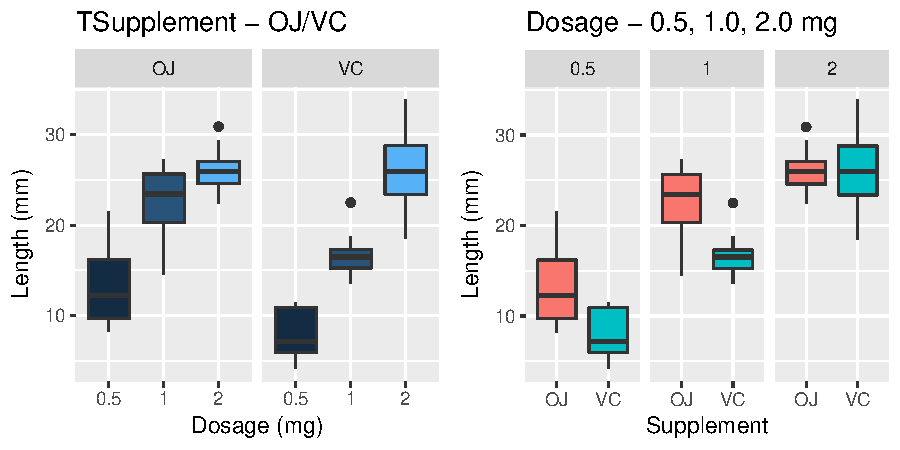
\includegraphics{Statistical_Inference_Project_2_files/figure-latex/unnamed-chunk-3-1.pdf}

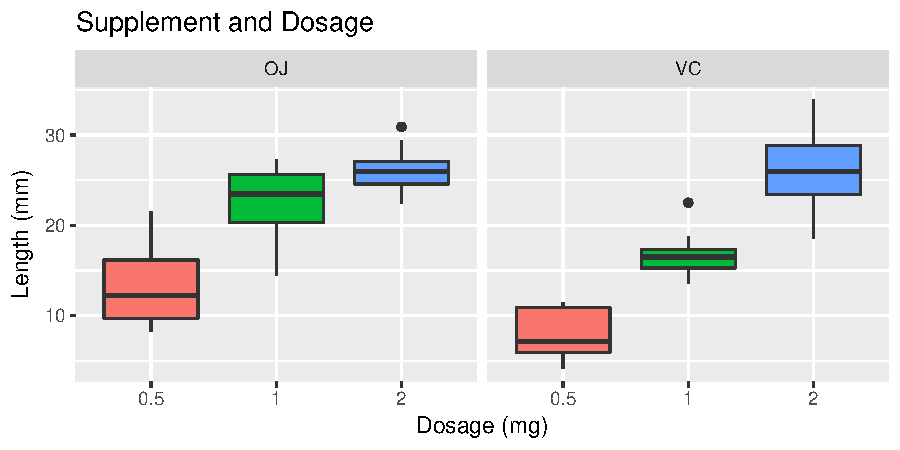
\includegraphics{Statistical_Inference_Project_2_files/figure-latex/unnamed-chunk-4-1.pdf}

\textbf{Inference from Plot 1:} The first box plot (LEFT) reveals that
average tooth growth with Orange juice is greater than the average tooth
growth than those which got their dose using Ascorbic acid (a form
Vitamin C).

\textbf{Inference from Plot 2:} The second box plot (RIGHT) also gives a
similar inference that the average tooth growth with Orange juice is
greater than the average tooth growth than those which got their dose
using Ascorbic acid (a form of Vitamin C). This plot also shows that the
diferences in tooth growth greater and the average length.

\textbf{Inference from Plot 3:} from the third plot (BOTTOM), the Orange
Juice group distribution is skewed to the left whereas the Ascorbic acid
group is fairly symmetric.

\subsection{Hypothesis Tests}\label{hypothesis-tests}

We will use the t distribution for our hypothesis tests and when
constructing confidence intervals.

We will have perform the t-tests to check if the p-value \textgreater{}
0.05 and if the confidence interval spans through 0.

First, we will perform the t-test based on \textbf{Supplement} Next, we
will perform the t-tests for each pair-wise combination of the dosage
levels

\textbf{Assumption:} We assume that the subjects were randomly assigned
to the groups and that they were sampled from a normal population.

\subsubsection{Supplement Type}\label{supplement-type}

\textbf{NULL Hypothesis:} We will consider that the average difference
in tooth length is 0, implying that the supplement type does not impact
the tooth growth.

We will first conduct t-test with unequal variances to check if the
difference in average tooth length between subjects who received their
dose using Orange juice and those who received their dose using Ascorbic
acid is statistically different from 0.

\begin{Shaded}
\begin{Highlighting}[]
\NormalTok{ttest_supp <-}\StringTok{ }\KeywordTok{t.test}\NormalTok{(len ~}\StringTok{ }\NormalTok{supp, ToothGrowth, }\DataTypeTok{var.equal =} \OtherTok{FALSE}\NormalTok{)}
\end{Highlighting}
\end{Shaded}

Following the values from the t-test,\\
- \textbf{p Value} = 0.061\\
- \textbf{confidence intervals:} {[}-0.1710156, 7.5710156{]}

The \textbf{p Value} = \textbf{0.061} is greater than the significance
level 0f 0.05 AND the confidence intervals contain 0.

We fail to reject the Null hypothesis.

\subsubsection{Dosage}\label{dosage}

We will have to perform t-test for every value of the dosage
administered (0.5, 1.0 and 2.0 mg) in three 3 pairwise comparisons (0.5,
1.0), (1.0,2.0) and (0.5,2.0) to determine if the dosage values impact
the tooth growth.

\textbf{NULL Hypothesis:} We will consider that the average difference
in tooth length is 0, implying that the Dosage does not impact the tooth
growth.

\begin{verbatim}
##              headinglabels         test1         test2         test3
## 1                  p Value  1.266297e-07  1.810829e-05  2.837553e-14
## 2  Confidence Interval-Low -1.198000e+01 -8.990000e+00 -1.815000e+01
## 3 Confidence Interval-High -6.280000e+00 -3.740000e+00 -1.284000e+01
\end{verbatim}

In each of the t-tests, we can see that the p value is very small, and
less than the significance level 0.5. Also the confidence intervals do
not include 0.

We can reject the Null hypothesis.

\subsubsection{Conclusion}\label{conclusion}

From the given sample data, we can infer that-\\
* The Supplement type, Orange juice of Ascorbic acid, does not impact
the tooth growth\\
* The dosage levels does impact the tooth growth

\subsection{Appendix (Source code)}\label{appendix-source-code}

Please find below the complete source code below.

\begin{Shaded}
\begin{Highlighting}[]
\CommentTok{# Load libraries for data processing and plotting}
\KeywordTok{library}\NormalTok{(ggplot2)}
\KeywordTok{library}\NormalTok{(datasets)}
\KeywordTok{library}\NormalTok{(gridExtra)}
\KeywordTok{library}\NormalTok{(grid)}

\CommentTok{# The Effect of Vitamin C on Tooth Growth in Guinea Pigs}
\KeywordTok{data}\NormalTok{(ToothGrowth)}

\KeywordTok{str}\NormalTok{(ToothGrowth)}

\CommentTok{# The below plot shows the tooth growth for }
\CommentTok{#    1) Each supplement types, }
\CommentTok{#    2) Dosage}
\CommentTok{#    3) Both (Dosage and Supplement)}

\NormalTok{p1 <-}\StringTok{ }\KeywordTok{ggplot}\NormalTok{(}\DataTypeTok{data=}\NormalTok{ToothGrowth, }\KeywordTok{aes}\NormalTok{(}\DataTypeTok{x=}\KeywordTok{factor}\NormalTok{(dose),}\DataTypeTok{y=}\NormalTok{len,}\DataTypeTok{fill=}\NormalTok{dose)) +}
\StringTok{     }\KeywordTok{geom_boxplot}\NormalTok{() +}
\StringTok{     }\KeywordTok{theme}\NormalTok{(}\DataTypeTok{legend.position=}\StringTok{"none"}\NormalTok{) +}\StringTok{ }
\StringTok{     }\KeywordTok{facet_grid}\NormalTok{(.~supp) +}
\StringTok{     }\KeywordTok{labs}\NormalTok{(}\DataTypeTok{title=}\StringTok{"TSupplement - OJ/VC"}\NormalTok{, }
          \DataTypeTok{x =} \StringTok{"Dosage (mg)"}\NormalTok{, }
          \DataTypeTok{y =} \StringTok{"Length (mm)"}\NormalTok{)}

\NormalTok{p2 <-}\StringTok{ }\KeywordTok{ggplot}\NormalTok{(}\DataTypeTok{data=}\NormalTok{ToothGrowth, }\KeywordTok{aes}\NormalTok{(}\DataTypeTok{x=}\NormalTok{supp,}\DataTypeTok{y=}\NormalTok{len,}\DataTypeTok{fill=}\NormalTok{supp)) +}
\StringTok{     }\KeywordTok{geom_boxplot}\NormalTok{() +}
\StringTok{     }\KeywordTok{theme}\NormalTok{(}\DataTypeTok{legend.position=}\StringTok{"none"}\NormalTok{) +}\StringTok{ }
\StringTok{     }\KeywordTok{facet_grid}\NormalTok{(.~dose)+}\StringTok{ }
\StringTok{     }\KeywordTok{labs}\NormalTok{(}\DataTypeTok{title=}\StringTok{"Dosage - 0.5, 1.0, 2.0 mg"}\NormalTok{, }
          \DataTypeTok{x =} \StringTok{"Supplement"}\NormalTok{, }
          \DataTypeTok{y =} \StringTok{"Length (mm)"}\NormalTok{)}

\NormalTok{p3<-}\StringTok{ }\KeywordTok{ggplot}\NormalTok{(ToothGrowth, }\KeywordTok{aes}\NormalTok{(}\KeywordTok{as.factor}\NormalTok{(dose), len)) +}
\StringTok{  }\KeywordTok{geom_boxplot}\NormalTok{(}\KeywordTok{aes}\NormalTok{(}\DataTypeTok{fill =} \KeywordTok{as.factor}\NormalTok{(dose))) +}\StringTok{ }
\StringTok{  }\KeywordTok{facet_grid}\NormalTok{(. ~}\StringTok{ }\NormalTok{supp) +}
\StringTok{  }\KeywordTok{xlab}\NormalTok{(}\StringTok{'Dosage (mg)'}\NormalTok{) +}
\StringTok{  }\KeywordTok{ylab}\NormalTok{(}\StringTok{'Length (mm)'}\NormalTok{) +}
\StringTok{  }\KeywordTok{ggtitle}\NormalTok{(}\StringTok{'Supplement and Dosage'}\NormalTok{) +}
\StringTok{  }\KeywordTok{theme}\NormalTok{(}\DataTypeTok{legend.position =} \StringTok{"none"}\NormalTok{)}

\KeywordTok{grid.newpage}\NormalTok{()}
\KeywordTok{pushViewport}\NormalTok{(}\KeywordTok{viewport}\NormalTok{(}\DataTypeTok{layout =} \KeywordTok{grid.layout}\NormalTok{(}\DecValTok{1}\NormalTok{,}\DecValTok{2}\NormalTok{, }\DataTypeTok{widths =} \KeywordTok{c}\NormalTok{(}\FloatTok{0.5}\NormalTok{, }\FloatTok{0.5}\NormalTok{))))}
\KeywordTok{print}\NormalTok{(p1, }\DataTypeTok{vp =} \KeywordTok{viewport}\NormalTok{(}\DataTypeTok{layout.pos.row =} \DecValTok{1}\NormalTok{, }\DataTypeTok{layout.pos.col =} \DecValTok{1}\NormalTok{))}
\KeywordTok{print}\NormalTok{(p2, }\DataTypeTok{vp =} \KeywordTok{viewport}\NormalTok{(}\DataTypeTok{layout.pos.row =} \DecValTok{1}\NormalTok{, }\DataTypeTok{layout.pos.col =} \DecValTok{2}\NormalTok{))}

\KeywordTok{print}\NormalTok{(p3)}

\CommentTok{# The t-test based on Supplement}
\NormalTok{ttest_supp <-}\StringTok{ }\KeywordTok{t.test}\NormalTok{(len ~}\StringTok{ }\NormalTok{supp, ToothGrowth, }\DataTypeTok{var.equal =} \OtherTok{FALSE}\NormalTok{)}

\CommentTok{# The t-tests for each pair-wise combination of the dosage levels}
\NormalTok{ttest_dose1<-}\KeywordTok{t.test}\NormalTok{(ToothGrowth$len[ToothGrowth$dose==}\FloatTok{0.5}\NormalTok{], }
                    \NormalTok{ToothGrowth$len[ToothGrowth$dose==}\DecValTok{1}\NormalTok{], }
                    \DataTypeTok{paired =} \OtherTok{FALSE}\NormalTok{, }\DataTypeTok{var.equal =} \OtherTok{TRUE}\NormalTok{)}

\NormalTok{ttest_dose2<-}\KeywordTok{t.test}\NormalTok{(ToothGrowth$len[ToothGrowth$dose==}\DecValTok{1}\NormalTok{], }
                    \NormalTok{ToothGrowth$len[ToothGrowth$dose==}\DecValTok{2}\NormalTok{], }
                    \DataTypeTok{paired =} \OtherTok{FALSE}\NormalTok{, }\DataTypeTok{var.equal =} \OtherTok{TRUE}\NormalTok{)}

\NormalTok{ttest_dose3<-}\KeywordTok{t.test}\NormalTok{(ToothGrowth$len[ToothGrowth$dose==}\FloatTok{0.5}\NormalTok{], }
                    \NormalTok{ToothGrowth$len[ToothGrowth$dose==}\DecValTok{2}\NormalTok{], }
                    \DataTypeTok{paired =} \OtherTok{FALSE}\NormalTok{, }\DataTypeTok{var.equal =} \OtherTok{TRUE}\NormalTok{)}

\CommentTok{# extract the right data and create a dataframe                 }
\NormalTok{test1 <-}\StringTok{ }\KeywordTok{c}\NormalTok{(ttest_dose1$p.value, }
           \KeywordTok{round}\NormalTok{(ttest_dose1$conf.int[}\DecValTok{1}\NormalTok{],}\DecValTok{2}\NormalTok{), }
           \KeywordTok{round}\NormalTok{(ttest_dose1$conf.int[}\DecValTok{2}\NormalTok{],}\DecValTok{2}\NormalTok{))}
\NormalTok{test2 <-}\StringTok{ }\KeywordTok{c}\NormalTok{(ttest_dose2$p.value, }
           \KeywordTok{round}\NormalTok{(ttest_dose2$conf.int[}\DecValTok{1}\NormalTok{],}\DecValTok{2}\NormalTok{), }
           \KeywordTok{round}\NormalTok{(ttest_dose2$conf.int[}\DecValTok{2}\NormalTok{],}\DecValTok{2}\NormalTok{))}
\NormalTok{test3 <-}\StringTok{ }\KeywordTok{c}\NormalTok{(ttest_dose3$p.value, }
           \KeywordTok{round}\NormalTok{(ttest_dose3$conf.int[}\DecValTok{1}\NormalTok{],}\DecValTok{2}\NormalTok{), }
           \KeywordTok{round}\NormalTok{(ttest_dose3$conf.int[}\DecValTok{2}\NormalTok{],}\DecValTok{2}\NormalTok{))}

\NormalTok{headinglabels <-}\StringTok{ }\KeywordTok{c}\NormalTok{(}\StringTok{"p Value"}\NormalTok{,}
                   \StringTok{"Confidence Interval-Low"}\NormalTok{,}
                   \StringTok{"Confidence Interval-High"}\NormalTok{)}

\NormalTok{test_df <-}\StringTok{ }\KeywordTok{data.frame}\NormalTok{(headinglabels,test1,test2,test3)}
\NormalTok{test_df}
\end{Highlighting}
\end{Shaded}


\end{document}
